\documentclass[11pt]{article}
\usepackage{colacl}
\usepackage{appendix}
\usepackage{graphicx}
\renewcommand{\appendixpagename}{\Large Appendices} %	10pt
\usepackage{listings}
\sloppy

\title{HPC Twitter GeoProcessing Report}
\author
{Zichun Zhu, Xiaoyue Ma}

\begin{document}
\maketitle


\section{Introduction}
This project explores geo information of twitters by classifying them into different Melbourne areas, and figures out the top 5 frequent hashtags in different area. In the report we will discuss the implementation of our parallelized program running on the University of Melbourne HPC facility SPARTAN. A brief description of how to identify Twitter usage and the top 5 hashtags from the given JSON files by using this application will be given.

There are four JSON files. The $melbGrid.json$ file illustrates the geographic information, and two small-size raw data files to test the application. After testing, it is necessary to search the total number of Twitter and the frequency of top-5 hashtags in each area from the $bigTwitter.json$ file.

What is more, 1 node and 1 core, 1 node and 8 cores, and 2 nodes and 8 cores with 4 cores per node are utilized.

\section{Methodology}

\subsection{HPC Parallelism}
In general there are two approaches to parallelize a program: divide work by data, and divide work by steps. The chosen is highly dependent on the specification of work. In geo processing, the number of steps per data entry is relatively small, while the size of whole data could be very large. Thus dividing work by data, and assigning works on a piece of data to different processes is more tractable.

\subsection{MPI}
There are different ways to classifiy parallel computers. The widely used classification, Flynn's taxonomy distinguishes computer architecture along instruction stream and data stream. According its definition, most current High Performance Computer(HPC) is in Multiple Instruction, Multiple Data(MIMD) type. Every process can work concurrently on different data stream, but those data and processors could be physically located in different place. To share the data between the processors,  we applied MPI in the implementation.

Message Passing Interface(MPI) is an useful open source tool in multi-core programming which contains many built-in functions to pass message between processes. The main difference between OpenMP and MPI is that the processes using MPI do not necessarily shared memory between each other, while OpenMP is a shared memory multiprocessing programming library.  MPI therefore able to be used in wide application regardless the physical architecture of platform.

\section{Brief Description of Project Design}
Two python files, $\_\_main\_\_.py$ and $reader.py$, are designed for both sequence and parallel computing.

\begin{figure}[h]
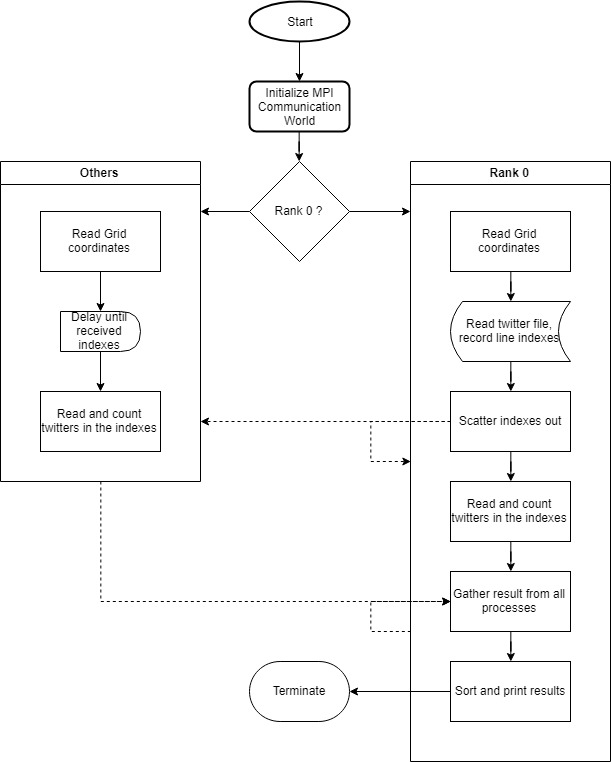
\includegraphics[width=0.48\textwidth]{process}
\caption{Flowchart}
\label{fig:flowchart}
\end{figure}

Figure \ref{fig:flowchart} shows the flowchart of our implementation.

What is more, considering that the size of data could be up to 15 GB, even though divided into chunks it is still a heavy load message transmission. So rather than reading the whole data and then sending out pieces of raw data, we let the master process scans and records the line indexes, and then scatters the indexes instead. A simple calculation can imply the efficiency and sufficiency. In $smallTwitter.json$, there are about 7000 lines, each is one tweet entry, and the size of the file is about 25 MB. If we assume tweets density in JSON file is even, a 15 GB file may contains: \[tweet\_num = 25MB / 15GB * 7000 \approx 4.2million\] If those tweets are represented in indexes, and each takes size of $int$\footnote{In Python, a $int$ takes 24 bytes.}, then 15 GB tweets file can be abstracted to: \[indexes\_size = 4.2million * 24bytes \approx 100MB \] The load of transmission could be largely reduced by simply representing tweets in form of indexes.

\section{Result}

As we can see from the Figure \ref{fig:Runtime Bar Chart} and the Table \ref{tab:Runtime Data}, after using parallel programming (1 node 8 tasks and 2 nodes 8 tasks), the speedup to searching $BigTwitter.json$ file is about 2.65 comparing with the serial one (1 node 1 task). And the two parallel programs are very similar, with only a slight time difference.

\begin{figure}[h]
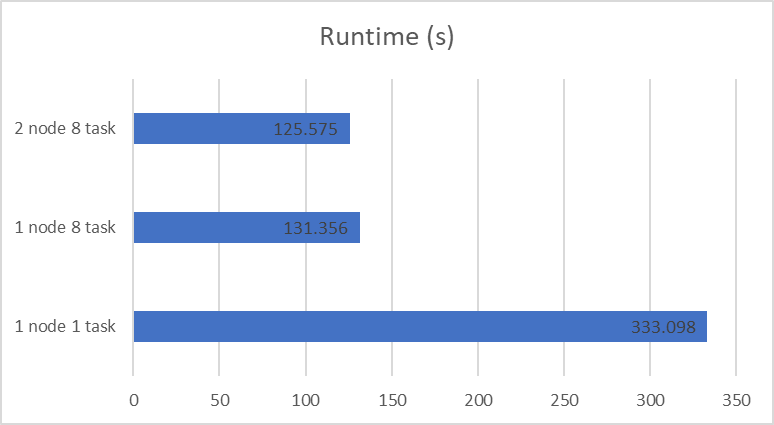
\includegraphics[width=0.48\textwidth]{runtimeChart2.png}
\caption{It is easy to observed that after using multiple cores the runtime is shortened more than half, but the impact from cores group arrangement is not significant.}
\label{fig:Runtime Bar Chart}
\end{figure}

\begin{table}[]
\begin{tabular}{c|ccc}
\multicolumn{1}{l|}{Run time(s)} & \multicolumn{1}{l}{Real} & \multicolumn{1}{l}{User} & \multicolumn{1}{l}{Sys} \\ \hline
1 Node 1 Task                   & 333.098                  & 320.854                  & 12.159                  \\ \hline
1 Node 8 Task                   & 131.356                  & 1029.688                & 17.667                  \\ \hline
2 Node 8 Task                   & 125.575                  & 350.427                  & 149.569
\end{tabular}
\caption{Runtime}
\label{tab:Runtime Data}
\end{table}

\begin{table}[]
\centering
\begin{tabular}{c|c}
\multicolumn{1}{l|}{} & \multicolumn{1}{l}{Speedup} \\ \hline
1 Node 1 Task         & 1                           \\ \hline
1 Node 8 Task         & 2.53                      \\ \hline
2 Node 8 Task         & 2.65                       
\end{tabular}
\caption{Speedup}
\label{tab:Speedup}
\end{table}

In the theory, according to Amdahl's law and the Gustafson-Basis’s law, with the increase of the processes, the speedup could be higher. And our experiments support it that 1 node 1 task, the non-parallel program costs more time to complete work on the same amount of data. Furthermore, the runtime between 2 nodes 8 task and 1 node 8 tasks, both parallel programs may similar, but due to the different communication bandwidth that the inter-communication within single node is faster than network communication among nodes, the 2 nodes 8 tasks one is supposed to spend more time than the 1 node 8 tasks one.

However, in practical the result shows 2 nodes 8 tasks has slightly less running time than 1 node 8 tasks. We make some hypothesises to explain this weird behaviour. Firstly, according the architecture of HPC the RAM in each node is physically shared among its jobs, there is no dedicate RAM for each process\footnote{In theory, dedicate RAM is possible to achieved but in this case our job Slurm script does not support.}, thus the inner channel bandwidth is shared by all processes. And also Slurm workload system allows one node running multiple jobs concurrently. So in our case, it is possible that in 1 node 8 tasks a single node is assigned 8 high memory throughput tasks which leads lack of channel bandwidth. On the other hand, in 2 nodes 8 tasks two node are assigned 4 tasks each and rest of cores may be in idle, so each node could be more relax and has ability to offer more resource to those 4 tasks. Moreover, since using of tweets' indexes, the time spend on MPI communication between processes is small. Therefore the difference between communication time within single node and communication time crossing two nodes could be neglected. 

And also, with the usage of line indexes, the communication time between processes could be shorten, thus, the time difference between within single node and cross two nodes could be neglected.

\section{Future Discussion}

Overall, multi-core programming gives us a noticeable speedup, but it is still very limited. Amdahl's law gives a criteria to  evaluate parallel programming efficiency: \[S=\frac{1}{a+(1-a)/N} \approx \frac{1}{a}\ for\ large\ N\] where $S$ is the speedup, $N$ is number of processors, and $a$ is the fraction of non-paralleled part over the whole program. Our experiment runs on 8 processors and the speedup is 2.65. Based on Amdahl's law the fraction of non-paralleled part is about 0.29. If we have an infinite number of processors, the speedup is converged to: \[S \approx \frac{1}{0.29} = 3.47\] It means that even if we are not limited on the number of processors, the speedup will never be higher than 3.47. The result is lower than expected, there is a potential issue we did not considered during implement.

The program may not gain any benefit from using of indexes in a system level. Abstracting indexes is definitely reduce the workload on MPI communication. However in meanwhile, multiple processors concurrently reads on the different positions of a same file may not reduce reading time, sometimes it even increases the reading time, because the mechanical nature of hard drive restricts its random access capacity. 


\begin{appendices}
\appendixpage
\section{Slurm Script}
\subsection{1 Node 1 Task}
\lstinputlisting[language=sh]{1node1task.slurm}
\subsection{1 Node 8 Task}
\lstinputlisting[language=sh]{1node8task.slurm}
\subsection{2 Node 8 Task}
\lstinputlisting[language=sh]{2node8task.slurm}
\end{appendices}

\end{document}
